\chapter{Evaluation}
\label{ch:Evaluation}

This section is used to interpret the data gathered in the analysis section and answer the two research questions \enquote{RQ1: Is there a difference between affective and discriminative touch for
both hands using the \gls{ost} encoding} and
\enquote{RQ2: Is there a significant
difference between using the \gls{ost} and the \gls{seq} encoding}.


\subsection{First Study}
%NASA TLX
In the first study, we compared the task load of the participants using the NASA TLX task load index. 

By analyzing the six different task load dimensions for each stimulus, and testing for significant differences between the stimuli, we found no significant differences. 

However, it is evident that there is a notable difference in the median performance statistics, suggesting that the \enquote{Performance} dimension was perceived more favourably in the stroking and vibration conditions.

%SELF ASSESSMENT
After completing the NASA TLX, participants were asked to self-assess how they perceived the stimulus on various dimensions, including \enquote{Feeling Pleasant}, \enquote{Helped Learning}, \enquote{Would Have Learned Faster}, \enquote{Would Use the Actuators to Support the Learning Process}, \enquote{Able to Understand Haptic Feedback}, and \enquote{Satisfaction Overall}, as depicted in \autoref{fig:questions_individual_firstStudy}.

A Kruskal-Wallis test was conducted on these responses. The results showed that the p-value for \enquote{Satisfaction} was $0.0504$. In combination with the effect size of $\eta^2$, this indicates a borderline significant difference, particularly for the tapping stimulus. Almost half of the participants rated it as very satisfying, resulting in a better Q1-Q3 quantile range compared to the other two stimuli. This suggests that participants were generally happier with the tapping stimulus, though the difference was not statistically significant.

Furthermore, the dimension \enquote{Would Have Learned Faster} yielded a p-value of $0.0882$ and an effect size of $0.1387$, which is also borderline significant, with more participants expressing dissatisfaction with the tapping stimulus.

%SELF DECISION
After the tests were completed, participants were asked to directly compare the stimuli and select which one they perceived as the best for each of the two dimensions: \enquote{Model Most Comfortable} and \enquote{Model That Helped Most in Learning}, as shown in \autoref{fig:questionsCompare-firstStudy}. 

The results indicate that the tapping and vibration stimuli were consistently rated better than the stroking stimulus in direct comparisons. In terms of comfort, both the tapping and vibration stimuli were perceived equally, while for learning, the tapping stimulus was preferred by $7/12$ of the participants. 

However, after conducting a \gls{csgf} and an \gls{emgf}, the results, presented in \autoref{table:statistical_tests_comparrisson_firstStudy}, reveal that the perceived differences between the stimuli were not statistically significant.

%COMMENTS
Participants were also asked to provide comments after the study. The comments received were as follows:

\enquote{Stroking is better than vibration, and tapping is better than stroking in both comfort and learning.}

\enquote{For vibration, it is sometimes difficult to identify which finger is vibrating.}\footnote{Translated from: \enquote{Bei Vibration ist manchmal schwer zu finden, welche Finger vibriert.}}

\enquote{The vibration was unclear, as it was difficult to tell which fingers were vibrating due to interference from other vibrators. The stroking was hard to feel.}

Lastly, \enquote{I think the tapping was the most comfortable, and I was able to distinguish the fingers. I sometimes couldn’t feel the stroker.}\footnote{Translated from: \enquote{Ich empfand den Tapper am angenehmsten und man konnte die Finger gut unterscheiden. Den Stroker habe ich manchmal nur kaum gespürt.}}

The participants' comments consistently indicate that tapping was preferred over stroking, followed by vibration. This preference seems to be due to stroking being difficult to feel and vibration being hard to distinguish. In contrast, tapping was favoured for its distinguishability.

%SUMARY    
In summary, we observed that performance was perceived as better for the stroking and vibration conditions in the NASA TLX. This is likely because the tapping actuator was more difficult to grasp, with an average of three fingers being stimulated for each character. This may have confused participants due to the number of taps involved.

The second questionnaire revealed that the tapping stimulus was borderline significant for \enquote{Satisfaction}, with participants rating it as the most satisfying. This finding is further supported by the comments provided by the users.

Interestingly, participants expressed dissatisfaction with the tapping stimulus in relation to \enquote{Would have learned faster}. This may stem from the same issue observed in the NASA TLX results—too much simultaneous stimulation.

However, in the \enquote{Helped learning} dimension, the tapping stimulus was still perceived as helpful, with nearly half of the participants rating it as very helpful for learning.

In a direct comparison of which stimulus was most helpful in learning, the tapping stimulus performed better. Additionally, its comfort level was rated similarly to the vibration stimulus, suggesting that from a qualitative perspective, it is a strong contender.

The vibration stimulus faced the issue of being difficult to distinguish, while the stroking stimulus generally performed worse. It was challenging to feel and distinguish and also underperformed in the \enquote{Helped learning} section of the usability questionnaire.



%  NASA TLX: \enquote{Performance} was perceived better for the stroking and vibration condition. 

% CUSTOM: \enquote{Satisfaction} (borderline significant) difference for the tapping stimulus, which is has with almost half of the participants voting it is very satisfying a better q1-q3 quantile range than the other two stimuli showing the users are rather happy with the tapping stimulus, however, not significant.

%  \enquote{Would have learned faster} with a pvalue of  $0.0882$ and a Effect size of $0.1387$ is borderline significant with more people dissattisfied with the tapping stimulus.

% COMPARE: It can be seen, taht the tapping and vibration Stimulus are in a direct comparison always better than the stroking one, while both, the tapping and vibration stimulus are the same for the comfortableness, moreover, the tapping was also with $7/12$ people perceiving it better in learning.

% COMMENTS:
% Tapping > Stroking > Vibration 
% vibration unclear, stroke hard to feel
% tapping distinguishable, stroking one hard to feel

%LEARNING TEST
For the objective data, we first gathered the results from all character learning tests, which are shown in \autoref{fig:learning_results_firstStudy}. After conducting Kruskal-Wallis tests for all the Braille characters, we found that there was no statistically significant difference between the sets, with the lowest p-value of $0.1599$ for the character \braille{b}(B). In this case, the stroking stimulus performed worse than the other two stimuli, but the results were essentially the same for the other stimuli.

The character \braille{d}(D) also showed a p-value of $0.2311$ with an effect size of $0.2663$, which is relatively high and reflects a slight difference. Here, the stroking stimulus was again perceived as slightly worse than the other stimuli; however, this difference was also far from statistically significance.

% B = stroking bad
% D = stroking bad

%WORD TEST
Lastly, we conducted a word test to assess performance with complete words after learning. The results are shown in \autoref{fig:test_results_firstStudy}. This analysis revealed that the stroking stimulus consistently performed worse for each word, followed by the tapping and vibration stimuli, which were similar for the word \braille{the} (THE). For the other two words, \braille{old} (OLD) and \braille{pub} (PUB), the median score was slightly better for the vibration stimulus, though the difference was small.

However, no statistical significance was found, as detailed in \autoref{table:significance_results_test_firstStudy}, where the lowest p-value was $0.1371$ for the word \braille{old} (OLD). It was also noted that there was always at least one participant who achieved the best score with tapping. In general, tapping performed better than the other two stimuli for the outliers, except for the word \braille{THE} (THE).

Vibration also performed well, ranking second for the words \braille{old} (OLD) and \braille{pub} (PUB) when considering the best performers.

% Stroking worse every time
% vibraiton best two times

After further analyzing the data, we found that for the \braille{l} (L) character, tapping performed the best, with no errors, followed by stroking, which also had some participants who made no errors.

For the \braille{b} (B) character, vibration outperformed both tapping and stroking, and this difference was borderline significant.

An interesting observation was that when all fingers on one hand needed to be stimulated, tapping appeared to be better than vibration, likely due to its higher distinguishability.

% L = tapping best (no errors), stroking words
% B = vibration l> tapping > strokign (For B borderline significant)

% General worst character is the E for all of the actuators, interesting because o looks similar in braille
% and for those characters all performed roughly the same bad

% when there are all fingers stimulate don one hand, tapping seems to be better than vibarion due to the distinguishability

%ERROR ANALYSIS

The error analysis revealed that the errors were mostly consistent across stimuli. For false negatives (FN), the most frequent error was \textcircled{1} [F], followed by \textcircled{3} [S] and \textcircled{5} [K] for both vibration and tapping and \textcircled{2} [D] and \textcircled{5} [K] for stroking. The least frequent false negative was \textcircled{6} [L].

The false positives (FP) also showed similar patterns. The most frequently added character was \textcircled{6} [L], while the least frequent false positive was \textcircled{1} [F].

This indicates that \textcircled{6} [L] was pressed almost constantly, even when not needed for some characters, while \textcircled{1} [F] was pressed less often and was mostly missed across all actuators.

%Detailled
A detailed analysis revealed that the errors were similar for both the vibration and stroking stimuli. For example, in the case of the character \braille{u}(U), the \textcircled{5} [K] key was pressed incorrectly for both stimuli. However, for the vibration stimulus, the \textcircled{4} [J] and \textcircled{2} [D] keys were also pressed incorrectly.

In terms of false negatives (FN), the \textcircled{6} [L] character was never missed with the vibration stimulus but was missed in 1/4 of the cases for tapping and stroking.

\subsection{Second Study}
The second study was conducted to see the differences between the different encodings \gls{ost} and \gls{seq}.

%NASA TLX
Similarly to the first study, we analyzed the subjective feelings of the participants using the NASA TLX, and the statistical significance of these results.

As shown in the plot and table, there is no significant difference between the two encodings, as measured by the Mann-Whitney U test (\gls{mwu}), with all p-values above 0.4.

This indicates that both encodings resulted in similar task load perceptions.
%same task load

%SELF ASSESSMENT
The self-assessment results of the participants and the corresponding significance tests, revealed no significant difference between the perceived quality of the different encodings, suggesting that they are essentially the same.

However, there is one notable difference in the \enquote{Feeling Pleasant} category, where the \gls{seq} encoding had a median of 3, while the \gls{ost} encoding scored a 4.

For the \enquote{Satisfaction} dimension, a larger difference can be observed in the Q1-Q3 quantile range, but this is attributed to one participant who rated the \gls{seq} encoding as more satisfying and did not provide a score of 3. Therefore, the encodings are effectively the same, as reflected by the p-value of 0.7 for this dimension.

%DIRECT COMPARE
The direct comparison, shown in \autoref{table:statistical_tests_comparrisson_secondStudy}, indicates that the \gls{seq} encoding was rated better for \enquote{Better distinguishable encoding} and \enquote{Helped learning encoding}, with 5/8 participants rating it higher for both categories. However, for \enquote{Most comfortable encoding}, the \gls{ost} encoding scored worse, with 3/8 participants rating it lower.

None of these differences were statistically significant, as indicated by the p-value of 0.4795 for all dimensions.

%SUMMARY
In general, there is no significant difference between the two encodings in terms of the participants' self-assessments. This is true for the task load measured by the NASA TLX and the self-assessment questionnaire, where neither dimension showed statistically significant differences.

Additionally, the direct comparison of which encoding was perceived as better after the study was not significant, as the differences were limited to just one participant per dimension. Therefore, none of the qualitative assessments showed significant differences.

%Learning results
After the characters were learned using one of the encodings, we conducted tests, with the Jaccard results shown in \autoref{fig:learning_results_secondStudy} and the results of the \gls{mwu} significance tests tabulated in \autoref{table:learning_significance_results_secondStudy_nonPar}.

An observed difference was tested using the character \braille{p}(P), which showed a Cohen's d effect size of $1.492$, with the \gls{seq} encoding performing better. For the character \braille{d}(D), the \gls{seq} encoding also performed better, with a median of 1 compared to the \gls{ost} encoding, which had a median of $0.425$.

For the characters \braille{l}(L) and \braille{u}(U), the \gls{ost} encoding performed better. Interestingly, for all Braille characters containing \textcircled{4} (J) or \textcircled{5} (K), the \gls{seq} encoding outperformed the \gls{ost}.


%TEST
After learning all the words, the word test was conducted, and the results are depicted in \autoref{fig:study2_test_results-firstStudy}. The significance tests are tabulated in \autoref{table:significance_results_test_secondStudy_nonPara}.

As seen from the significance tests, with p-values over 0.7, there is no significant difference between the encodings. Additionally, the plot shows that the worst-performing \gls{seq} encoding performed worse for both words than the worst-performing \gls{ost} encoding. However, the best-performing \gls{seq} encodings resulted in slightly better participant scores than the best \gls{ost} encodings, indicating a wider variance in performance.

%CHARACTER ANALYSE
We then analyzed the individual characters as before, which are plotted in \autoref{fig:f1score_test_study2}, with their significance tests tabulated in \autoref{table:learning_significance_results_secondStudy_nonPar}.

As shown, there are larger differences for the characters \braille{b}(B), \braille{p}(P), \braille{l}(L), and \braille{d}(D); however, none of these differences were statistically significant.


%ERRORS
We then tested the false positives (FP) and false negatives (FN) for each of the characters, as shown in \autoref{fig:missedSurplus_study2}.

The results indicate that many FN errors were associated with \textcircled{3} [S]. For the FP errors, both encodings showed \textcircled{2} [D], \textcircled{5} [K], and \textcircled{6} [L].

%CHARACTER CHECKS
We then analyzed the errors for each character, with the plots available in \autoref{fig:missed_surplus_percentages_study2} for both the \gls{seq} and \gls{ost} encodings.

The analysis of the plots revealed differences for FP in the characters \braille{b}(B), \braille{l}(L), and \braille{d}(D). For FN, the differences were observed in the characters \braille{o}(O), \braille{l}(L), \braille{p}(P), and \braille{b}(B).

The largest differences for FN were seen with the Braille character \braille{p}(P), where the keys \textcircled{3} [S] and \textcircled{1} [F] were often missed. For FP, the largest differences were with the Braille character \braille{b}(B), where the keys \textcircled{3} [S] and \textcircled{5} [K] were pressed too frequently.

%COMMENTS
The comments evaluating the different encoding schemes were:
\enquote{For OST, I don't perceive the vibration as accurately.},
\enquote{I had difficulties to register which finger did vibrate.},
\enquote{If I had to learn with one method with the goal of having learned something in the end, I would choose SEQ. If it's just for fun, I would choose OST.},
\enquote{I had difficulties to register which finger did vibrate.},
\enquote{OST was easier to ignore. SEQ was harder to ignore, more irritating during the game.},
\enquote{In the second section, I learned the Braille better because the devices of each finger didn’t vibrate at the same time.},
This shows that the users seem to prefer the \gls{seq} encoding over the \gls{ost} by saying it is more distinguishable.


\subsection{Threats to validity}
\section{Threats to Validity}

We identified several potential threats to validity in both of our studies, which are categorized into internal, external, and construct validity, following the framework outlined by Lago et al. \cite{10.1145/3674805.3686691} which are illustrated in \autoref{fig:threats_to_validity}.

\subsection{Internal Validity}
One key threat to internal validity is the sample size. In the \textbf{first study}, an \textit{a priori} power analysis using the g* power software determined that a sample size of \textbf{36} was required to achieve \textbf{80\% power}. However, only \textbf{12} samples were used, and a \textit{post hoc} power analysis revealed an achieved power of only \textbf{0.34}. This low statistical power increases the risk of a \textbf{Type II error}, meaning that true effects may not have been detected. 

Similarly, in the \textbf{second study}, the \textit{a priori} power analysis indicated that a sample size of \textbf{45} was necessary for adequate statistical power. However, the \textit{post hoc} power analysis showed that the actual power achieved was only \textbf{0.356}. These findings suggest that both studies were underpowered, limiting the reliability of their conclusions.

Additionally, we used a relatively young participant group, with a median age of \textbf{28.67 years} in the first study and \textbf{24.5 years} in the second study. Both studies also included only \textbf{one left-handed participant}. Furthermore, the gender distribution was imbalanced, with only \textbf{three female participants} in each study. This lack of diversity may limit the generalizability of our findings across different populations.

\subsection{External and Construct Validity}
Hand size emerged as a potential factor affecting external and construct validity. Differences in hand size may influence the placement of actuators, as they could sit differently on individuals with larger or smaller hands. This variation in actuator positioning could have introduced slight inconsistencies in the stimuli delivered, potentially influencing our results.

Another construct validity concern relates to stimulus perception. Some participants reported that they did not perceive the \textbf{stroking stimulus} as effectively as the \textbf{vibration} or \textbf{tapping} stimuli. This perception discrepancy could impact the interpretation of the stimulus' effects and must be considered when evaluating the results.

Lastly, none of the participants were native English speakers. Although the words used in the experiments were simple, short, and commonly encountered, some participants may have had minor spelling difficulties. However, we consider this issue to have a negligible impact on the findings.

\begin{figure}
    \centering
    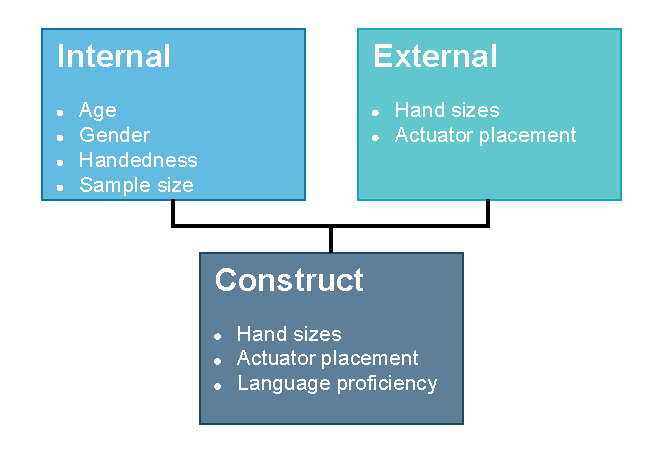
\includegraphics[width=0.5\linewidth]{src/pictures/StudyData/Threats_to_validity.drawio.pdf}
    \caption{Threats to validity}
    \label{fig:threats_to_validity}
\end{figure}




